% Options for packages loaded elsewhere
\PassOptionsToPackage{unicode}{hyperref}
\PassOptionsToPackage{hyphens}{url}
\PassOptionsToPackage{dvipsnames,svgnames,x11names}{xcolor}
%
\documentclass[
  letterpaper,
  DIV=11,
  numbers=noendperiod]{scrartcl}

\usepackage{amsmath,amssymb}
\usepackage{iftex}
\ifPDFTeX
  \usepackage[T1]{fontenc}
  \usepackage[utf8]{inputenc}
  \usepackage{textcomp} % provide euro and other symbols
\else % if luatex or xetex
  \usepackage{unicode-math}
  \defaultfontfeatures{Scale=MatchLowercase}
  \defaultfontfeatures[\rmfamily]{Ligatures=TeX,Scale=1}
\fi
\usepackage{lmodern}
\ifPDFTeX\else  
    % xetex/luatex font selection
\fi
% Use upquote if available, for straight quotes in verbatim environments
\IfFileExists{upquote.sty}{\usepackage{upquote}}{}
\IfFileExists{microtype.sty}{% use microtype if available
  \usepackage[]{microtype}
  \UseMicrotypeSet[protrusion]{basicmath} % disable protrusion for tt fonts
}{}
\makeatletter
\@ifundefined{KOMAClassName}{% if non-KOMA class
  \IfFileExists{parskip.sty}{%
    \usepackage{parskip}
  }{% else
    \setlength{\parindent}{0pt}
    \setlength{\parskip}{6pt plus 2pt minus 1pt}}
}{% if KOMA class
  \KOMAoptions{parskip=half}}
\makeatother
\usepackage{xcolor}
\setlength{\emergencystretch}{3em} % prevent overfull lines
\setcounter{secnumdepth}{-\maxdimen} % remove section numbering
% Make \paragraph and \subparagraph free-standing
\makeatletter
\ifx\paragraph\undefined\else
  \let\oldparagraph\paragraph
  \renewcommand{\paragraph}{
    \@ifstar
      \xxxParagraphStar
      \xxxParagraphNoStar
  }
  \newcommand{\xxxParagraphStar}[1]{\oldparagraph*{#1}\mbox{}}
  \newcommand{\xxxParagraphNoStar}[1]{\oldparagraph{#1}\mbox{}}
\fi
\ifx\subparagraph\undefined\else
  \let\oldsubparagraph\subparagraph
  \renewcommand{\subparagraph}{
    \@ifstar
      \xxxSubParagraphStar
      \xxxSubParagraphNoStar
  }
  \newcommand{\xxxSubParagraphStar}[1]{\oldsubparagraph*{#1}\mbox{}}
  \newcommand{\xxxSubParagraphNoStar}[1]{\oldsubparagraph{#1}\mbox{}}
\fi
\makeatother

\usepackage{color}
\usepackage{fancyvrb}
\newcommand{\VerbBar}{|}
\newcommand{\VERB}{\Verb[commandchars=\\\{\}]}
\DefineVerbatimEnvironment{Highlighting}{Verbatim}{commandchars=\\\{\}}
% Add ',fontsize=\small' for more characters per line
\usepackage{framed}
\definecolor{shadecolor}{RGB}{241,243,245}
\newenvironment{Shaded}{\begin{snugshade}}{\end{snugshade}}
\newcommand{\AlertTok}[1]{\textcolor[rgb]{0.68,0.00,0.00}{#1}}
\newcommand{\AnnotationTok}[1]{\textcolor[rgb]{0.37,0.37,0.37}{#1}}
\newcommand{\AttributeTok}[1]{\textcolor[rgb]{0.40,0.45,0.13}{#1}}
\newcommand{\BaseNTok}[1]{\textcolor[rgb]{0.68,0.00,0.00}{#1}}
\newcommand{\BuiltInTok}[1]{\textcolor[rgb]{0.00,0.23,0.31}{#1}}
\newcommand{\CharTok}[1]{\textcolor[rgb]{0.13,0.47,0.30}{#1}}
\newcommand{\CommentTok}[1]{\textcolor[rgb]{0.37,0.37,0.37}{#1}}
\newcommand{\CommentVarTok}[1]{\textcolor[rgb]{0.37,0.37,0.37}{\textit{#1}}}
\newcommand{\ConstantTok}[1]{\textcolor[rgb]{0.56,0.35,0.01}{#1}}
\newcommand{\ControlFlowTok}[1]{\textcolor[rgb]{0.00,0.23,0.31}{\textbf{#1}}}
\newcommand{\DataTypeTok}[1]{\textcolor[rgb]{0.68,0.00,0.00}{#1}}
\newcommand{\DecValTok}[1]{\textcolor[rgb]{0.68,0.00,0.00}{#1}}
\newcommand{\DocumentationTok}[1]{\textcolor[rgb]{0.37,0.37,0.37}{\textit{#1}}}
\newcommand{\ErrorTok}[1]{\textcolor[rgb]{0.68,0.00,0.00}{#1}}
\newcommand{\ExtensionTok}[1]{\textcolor[rgb]{0.00,0.23,0.31}{#1}}
\newcommand{\FloatTok}[1]{\textcolor[rgb]{0.68,0.00,0.00}{#1}}
\newcommand{\FunctionTok}[1]{\textcolor[rgb]{0.28,0.35,0.67}{#1}}
\newcommand{\ImportTok}[1]{\textcolor[rgb]{0.00,0.46,0.62}{#1}}
\newcommand{\InformationTok}[1]{\textcolor[rgb]{0.37,0.37,0.37}{#1}}
\newcommand{\KeywordTok}[1]{\textcolor[rgb]{0.00,0.23,0.31}{\textbf{#1}}}
\newcommand{\NormalTok}[1]{\textcolor[rgb]{0.00,0.23,0.31}{#1}}
\newcommand{\OperatorTok}[1]{\textcolor[rgb]{0.37,0.37,0.37}{#1}}
\newcommand{\OtherTok}[1]{\textcolor[rgb]{0.00,0.23,0.31}{#1}}
\newcommand{\PreprocessorTok}[1]{\textcolor[rgb]{0.68,0.00,0.00}{#1}}
\newcommand{\RegionMarkerTok}[1]{\textcolor[rgb]{0.00,0.23,0.31}{#1}}
\newcommand{\SpecialCharTok}[1]{\textcolor[rgb]{0.37,0.37,0.37}{#1}}
\newcommand{\SpecialStringTok}[1]{\textcolor[rgb]{0.13,0.47,0.30}{#1}}
\newcommand{\StringTok}[1]{\textcolor[rgb]{0.13,0.47,0.30}{#1}}
\newcommand{\VariableTok}[1]{\textcolor[rgb]{0.07,0.07,0.07}{#1}}
\newcommand{\VerbatimStringTok}[1]{\textcolor[rgb]{0.13,0.47,0.30}{#1}}
\newcommand{\WarningTok}[1]{\textcolor[rgb]{0.37,0.37,0.37}{\textit{#1}}}

\providecommand{\tightlist}{%
  \setlength{\itemsep}{0pt}\setlength{\parskip}{0pt}}\usepackage{longtable,booktabs,array}
\usepackage{calc} % for calculating minipage widths
% Correct order of tables after \paragraph or \subparagraph
\usepackage{etoolbox}
\makeatletter
\patchcmd\longtable{\par}{\if@noskipsec\mbox{}\fi\par}{}{}
\makeatother
% Allow footnotes in longtable head/foot
\IfFileExists{footnotehyper.sty}{\usepackage{footnotehyper}}{\usepackage{footnote}}
\makesavenoteenv{longtable}
\usepackage{graphicx}
\makeatletter
\def\maxwidth{\ifdim\Gin@nat@width>\linewidth\linewidth\else\Gin@nat@width\fi}
\def\maxheight{\ifdim\Gin@nat@height>\textheight\textheight\else\Gin@nat@height\fi}
\makeatother
% Scale images if necessary, so that they will not overflow the page
% margins by default, and it is still possible to overwrite the defaults
% using explicit options in \includegraphics[width, height, ...]{}
\setkeys{Gin}{width=\maxwidth,height=\maxheight,keepaspectratio}
% Set default figure placement to htbp
\makeatletter
\def\fps@figure{htbp}
\makeatother
% definitions for citeproc citations
\NewDocumentCommand\citeproctext{}{}
\NewDocumentCommand\citeproc{mm}{%
  \begingroup\def\citeproctext{#2}\cite{#1}\endgroup}
\makeatletter
 % allow citations to break across lines
 \let\@cite@ofmt\@firstofone
 % avoid brackets around text for \cite:
 \def\@biblabel#1{}
 \def\@cite#1#2{{#1\if@tempswa , #2\fi}}
\makeatother
\newlength{\cslhangindent}
\setlength{\cslhangindent}{1.5em}
\newlength{\csllabelwidth}
\setlength{\csllabelwidth}{3em}
\newenvironment{CSLReferences}[2] % #1 hanging-indent, #2 entry-spacing
 {\begin{list}{}{%
  \setlength{\itemindent}{0pt}
  \setlength{\leftmargin}{0pt}
  \setlength{\parsep}{0pt}
  % turn on hanging indent if param 1 is 1
  \ifodd #1
   \setlength{\leftmargin}{\cslhangindent}
   \setlength{\itemindent}{-1\cslhangindent}
  \fi
  % set entry spacing
  \setlength{\itemsep}{#2\baselineskip}}}
 {\end{list}}
\usepackage{calc}
\newcommand{\CSLBlock}[1]{\hfill\break\parbox[t]{\linewidth}{\strut\ignorespaces#1\strut}}
\newcommand{\CSLLeftMargin}[1]{\parbox[t]{\csllabelwidth}{\strut#1\strut}}
\newcommand{\CSLRightInline}[1]{\parbox[t]{\linewidth - \csllabelwidth}{\strut#1\strut}}
\newcommand{\CSLIndent}[1]{\hspace{\cslhangindent}#1}

\KOMAoption{captions}{tableheading}
\usepackage{amsmath}
\usepackage{amssymb}
\makeatletter
\@ifpackageloaded{tcolorbox}{}{\usepackage[skins,breakable]{tcolorbox}}
\@ifpackageloaded{fontawesome5}{}{\usepackage{fontawesome5}}
\definecolor{quarto-callout-color}{HTML}{909090}
\definecolor{quarto-callout-note-color}{HTML}{0758E5}
\definecolor{quarto-callout-important-color}{HTML}{CC1914}
\definecolor{quarto-callout-warning-color}{HTML}{EB9113}
\definecolor{quarto-callout-tip-color}{HTML}{00A047}
\definecolor{quarto-callout-caution-color}{HTML}{FC5300}
\definecolor{quarto-callout-color-frame}{HTML}{acacac}
\definecolor{quarto-callout-note-color-frame}{HTML}{4582ec}
\definecolor{quarto-callout-important-color-frame}{HTML}{d9534f}
\definecolor{quarto-callout-warning-color-frame}{HTML}{f0ad4e}
\definecolor{quarto-callout-tip-color-frame}{HTML}{02b875}
\definecolor{quarto-callout-caution-color-frame}{HTML}{fd7e14}
\makeatother
\makeatletter
\@ifpackageloaded{caption}{}{\usepackage{caption}}
\AtBeginDocument{%
\ifdefined\contentsname
  \renewcommand*\contentsname{Table of contents}
\else
  \newcommand\contentsname{Table of contents}
\fi
\ifdefined\listfigurename
  \renewcommand*\listfigurename{List of Figures}
\else
  \newcommand\listfigurename{List of Figures}
\fi
\ifdefined\listtablename
  \renewcommand*\listtablename{List of Tables}
\else
  \newcommand\listtablename{List of Tables}
\fi
\ifdefined\figurename
  \renewcommand*\figurename{Figure}
\else
  \newcommand\figurename{Figure}
\fi
\ifdefined\tablename
  \renewcommand*\tablename{Table}
\else
  \newcommand\tablename{Table}
\fi
}
\@ifpackageloaded{float}{}{\usepackage{float}}
\floatstyle{ruled}
\@ifundefined{c@chapter}{\newfloat{codelisting}{h}{lop}}{\newfloat{codelisting}{h}{lop}[chapter]}
\floatname{codelisting}{Listing}
\newcommand*\listoflistings{\listof{codelisting}{List of Listings}}
\makeatother
\makeatletter
\makeatother
\makeatletter
\@ifpackageloaded{caption}{}{\usepackage{caption}}
\@ifpackageloaded{subcaption}{}{\usepackage{subcaption}}
\makeatother

\ifLuaTeX
  \usepackage{selnolig}  % disable illegal ligatures
\fi
\usepackage{bookmark}

\IfFileExists{xurl.sty}{\usepackage{xurl}}{} % add URL line breaks if available
\urlstyle{same} % disable monospaced font for URLs
\hypersetup{
  pdftitle={R2D2 Prior},
  colorlinks=true,
  linkcolor={blue},
  filecolor={Maroon},
  citecolor={Blue},
  urlcolor={Blue},
  pdfcreator={LaTeX via pandoc}}


\title{R2D2 Prior}
\author{}
\date{}

\begin{document}
\maketitle


\subsection{General Principles}\label{general-principles}

Rather than setting arbitrary, independent variances for individual
regression coefficients --- which can be difficult to intuit --- the
\textbf{R2D2} (\emph{R}-squared induced Dirichlet Decomposition) prior
places a prior directly on a macro-level, easily interpretable metric:
the model's overall goodness-of-fit, \(R^2\). This prior was introduced
in (\textbf{gelman2022r2d2?}).

Think of it as a \textbf{variance budget}. A single prior on \(R^2\)
opens a pot of ``explained variance''; a Dirichlet simplex then divides
that pot among the predictors; each predictor's slice becomes the prior
variance of its coefficient. The generative process has five steps
(Figure~\ref{fig-r2d2}):

\begin{figure}

\centering{

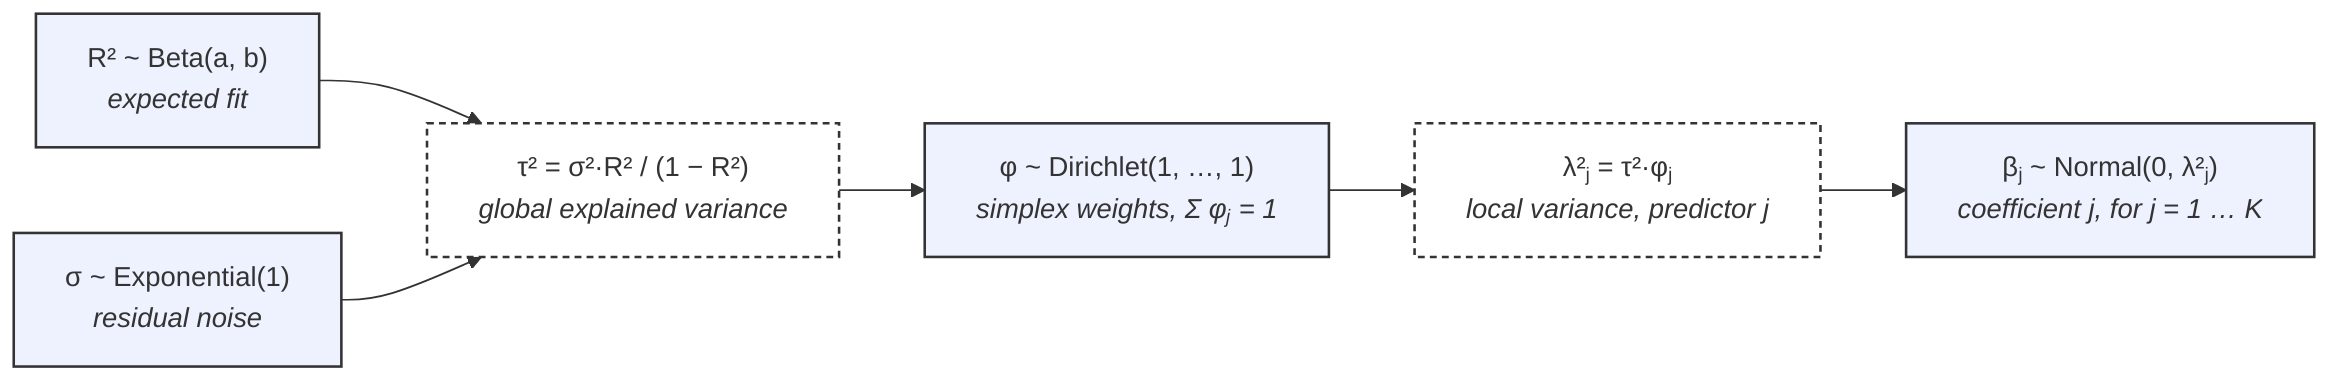
\includegraphics[width=1\textwidth,height=\textheight]{Figures/R2D2_hierarchy.png}

}

\caption{\label{fig-r2d2}The R2D2 prior as a variance budget: a Beta
prior on \(R^2\) --- together with the residual scale \(\sigma\) ---
opens a global explained variance \(\tau^2\); a flat Dirichlet splits it
into per-predictor weights \(\phi_j\); and each slice
\(\lambda_j^2 = \tau^2\phi_j\) becomes the prior variance of coefficient
\(\beta_j\). Dashed nodes are deterministic transforms.}

\end{figure}%

\begin{enumerate}
\def\labelenumi{\arabic{enumi}.}
\item
  \textbf{Set the expectation.} \(R^2 \sim \text{Beta}(a, b)\) --- how
  much of \(y\)'s variance do you expect this model to explain? The
  conservative default is \(\text{Beta}(1/3, 3)\) (prior mean
  \(R^2 = 0.1\)).
\item
  \textbf{Open the budget.} \(\tau^2 = \dfrac{\sigma^2 R^2}{1 - R^2}\)
  maps the \(R^2\) belief onto a total signal variance, scaled by the
  residual variance \(\sigma^2\). This \(\tau^2\) is the signal-to-noise
  budget available to the coefficients (see
  \hyperref[sec-r2-definition]{\emph{Definition of \(R^2\)}} for the
  exact quantity \(R^2\) refers to).
\item
  \textbf{Split it.} \(\phi \sim \text{Dirichlet}(a_0, \dots, a_0)\) is
  a vector of \(K\) non-negative weights that sum to one. The
  concentration \(a_0\) controls how sparse the split is: \(a_0 = 1\)
  (the usual default) gives every predictor the same prior share ---
  ridge-like --- while \(a_0 < 1\) favours allocating the budget to a
  few predictors, which makes the induced coefficient priors
  heavier-tailed and more horseshoe-like.
\item
  \textbf{Hand out slices.} \(\lambda_j^2 = \tau^2 \phi_j\) is predictor
  \(j\)'s share of the budget.
\item
  \textbf{Draw the coefficient.}
  \(\beta_j \sim \text{Normal}(0, \lambda_j^2)\).
\end{enumerate}

\begin{tcolorbox}[enhanced jigsaw, titlerule=0mm, arc=.35mm, leftrule=.75mm, colback=white, bottomtitle=1mm, toptitle=1mm, colbacktitle=quarto-callout-note-color!10!white, colframe=quarto-callout-note-color-frame, opacitybacktitle=0.6, bottomrule=.15mm, opacityback=0, toprule=.15mm, left=2mm, title=\textcolor{quarto-callout-note-color}{\faInfo}\hspace{0.5em}{Note}, rightrule=.15mm, breakable, coltitle=black]

\textbf{The budget metaphor.} Because the Dirichlet weights sum to one,
the predictors \emph{compete} for a fixed pot: a predictor that claims a
large share leaves less for the rest, so unsupported predictors are
handed a tiny \(\phi_j\) and their coefficients collapse toward zero ---
adaptive sparsity without an explicit spike-at-zero. This reading only
holds if the predictors are \textbf{standardized}:
\(\lambda_j^2 = \tau^2\phi_j\) distributes \emph{variance}, so
predictors on incomparable scales would confound ``share of explained
variance'' with unit of measurement.

\end{tcolorbox}

\subsection{Considerations}\label{considerations}

\begin{tcolorbox}[enhanced jigsaw, titlerule=0mm, arc=.35mm, leftrule=.75mm, colback=white, bottomtitle=1mm, toptitle=1mm, colbacktitle=quarto-callout-note-color!10!white, colframe=quarto-callout-note-color-frame, opacitybacktitle=0.6, bottomrule=.15mm, opacityback=0, toprule=.15mm, left=2mm, title=\textcolor{quarto-callout-note-color}{\faInfo}\hspace{0.5em}{Note}, rightrule=.15mm, breakable, coltitle=black]

\begin{itemize}
\item
  Instead of declaring independent \phantomsection\label{prior}{{prior
  distributions 🛈}} for each coefficient variance, the R2D2 prior
  encodes a single macro-level belief: the fraction of the outcome
  variance the model is expected to explain. Eliciting expert knowledge
  on an expected \(R^2\) is much easier than guessing the variance of an
  abstract regression weight.
\item
  Because the Dirichlet weights \(\phi_j\) must sum to one, the
  predictors are forced to ``compete'' for a share of the total
  variance. If one predictor takes a larger share, the others are
  inherently penalized. This \emph{adaptive sparsity} naturally shrinks
  irrelevant variables towards zero and helps prevent overfitting.
\item
  The induced coefficient priors concentrate probability mass around
  zero while maintaining heavy tails: noise is strongly regularized, yet
  genuinely large coefficients are estimated without bias.
\item
  The framework extends to
  \href{15.\%20Varying\%20intercepts.qmd}{varying intercepts} and other
  \href{15.\%20Varying\%20intercepts.qmd}{{hierarchical 🛈}} models: the
  simplex is expanded so that the variance components of the grouping
  factors receive their own slice of the global variance \(\tau^2\),
  forcing fixed covariates and group-level effects to compete for the
  total explained variance.
\item
  In mixed-effects models, the Beta prior must target the
  \emph{conditional} \(R^2\) (variance explained by fixed plus varying
  effects), not the \emph{marginal} \(R^2\) (fixed effects alone), so
  that the full signal-to-noise ratio is captured before the Dirichlet
  weights decompose it down the hierarchy.
\end{itemize}

\end{tcolorbox}

\subsection{Example}\label{example}

Below is an example code snippet demonstrating an \emph{R2D2 prior} on
the regression coefficients using the Bayesian Inference (\textbf{BI})
package. A Beta prior on the expected \(R^2\) is transformed into a
global variance, which is then decomposed through a Dirichlet simplex
into local variances for each of the two predictors (weight and age).
This example is based on (\textbf{gelman2022r2d2?}).

\subsection{Python}

\begin{Shaded}
\begin{Highlighting}[]
\ImportTok{from}\NormalTok{ BayesForge }\ImportTok{import}\NormalTok{ bf}
\ImportTok{import}\NormalTok{ jax.numpy }\ImportTok{as}\NormalTok{ jnp}

\CommentTok{\# Setup device{-}{-}{-}{-}{-}{-}{-}{-}{-}{-}{-}{-}{-}{-}{-}{-}{-}{-}{-}{-}{-}{-}{-}{-}{-}{-}{-}{-}{-}{-}{-}{-}{-}{-}{-}{-}{-}{-}{-}{-}{-}{-}{-}{-}{-}{-}{-}{-}}
\NormalTok{m }\OperatorTok{=}\NormalTok{ bf(platform}\OperatorTok{=}\StringTok{"cpu"}\NormalTok{)}

\CommentTok{\# Import Data \& Data Manipulation {-}{-}{-}{-}{-}{-}{-}{-}{-}{-}{-}{-}{-}{-}{-}{-}{-}{-}{-}{-}{-}{-}{-}{-}{-}{-}{-}{-}{-}{-}{-}{-}{-}{-}{-}{-}{-}{-}{-}{-}{-}{-}{-}{-}{-}{-}{-}{-}}
\CommentTok{\# Import}
\NormalTok{data\_path }\OperatorTok{=}\NormalTok{ m.load.howell1(only\_path}\OperatorTok{=}\VariableTok{True}\NormalTok{)}
\NormalTok{m.data(data\_path, sep}\OperatorTok{=}\StringTok{";"}\NormalTok{)}
\NormalTok{m.df }\OperatorTok{=}\NormalTok{ m.df[m.df.age }\OperatorTok{\textgreater{}} \DecValTok{18}\NormalTok{]  }\CommentTok{\# Subset data to adults}
\NormalTok{m.scale([}\StringTok{"weight"}\NormalTok{, }\StringTok{"age"}\NormalTok{])  }\CommentTok{\# Normalize}

\CommentTok{\# Define model {-}{-}{-}{-}{-}{-}{-}{-}{-}{-}{-}{-}{-}{-}{-}{-}{-}{-}{-}{-}{-}{-}{-}{-}{-}{-}{-}{-}{-}{-}{-}{-}{-}{-}{-}{-}{-}{-}{-}{-}{-}{-}{-}{-}{-}{-}{-}{-}}
\KeywordTok{def}\NormalTok{ model(height, weight, age):}
    \CommentTok{\# R2D2 prior: Beta prior on the expected R\^{}2 of the model}
\NormalTok{    r2 }\OperatorTok{=}\NormalTok{ m.dist.beta(}\DecValTok{1} \OperatorTok{/} \DecValTok{3}\NormalTok{, }\DecValTok{3}\NormalTok{, name}\OperatorTok{=}\StringTok{"r2"}\NormalTok{)}
\NormalTok{    sigma }\OperatorTok{=}\NormalTok{ m.dist.exponential(}\DecValTok{1}\NormalTok{, name}\OperatorTok{=}\StringTok{"s"}\NormalTok{)}
    \CommentTok{\# Global (total explained) variance}
\NormalTok{    tau2 }\OperatorTok{=}\NormalTok{ sigma}\OperatorTok{**}\DecValTok{2} \OperatorTok{*}\NormalTok{ r2 }\OperatorTok{/}\NormalTok{ (}\DecValTok{1} \OperatorTok{{-}}\NormalTok{ r2)}
    \CommentTok{\# Dirichlet weights over the K = 2 predictors}
\NormalTok{    phi }\OperatorTok{=}\NormalTok{ m.dist.dirichlet(jnp.ones(}\DecValTok{2}\NormalTok{), name}\OperatorTok{=}\StringTok{"phi"}\NormalTok{)}
    \CommentTok{\# Local coefficient variances}
\NormalTok{    lam2 }\OperatorTok{=}\NormalTok{ tau2 }\OperatorTok{*}\NormalTok{ phi}
    \CommentTok{\# Parameter prior distributions}
\NormalTok{    alpha }\OperatorTok{=}\NormalTok{ m.dist.normal(}\DecValTok{0}\NormalTok{, }\FloatTok{0.5}\NormalTok{, name}\OperatorTok{=}\StringTok{"alpha"}\NormalTok{)}
\NormalTok{    beta1 }\OperatorTok{=}\NormalTok{ m.dist.normal(}\DecValTok{0}\NormalTok{, jnp.sqrt(lam2[}\DecValTok{0}\NormalTok{]), name}\OperatorTok{=}\StringTok{"beta1"}\NormalTok{)}
\NormalTok{    beta2 }\OperatorTok{=}\NormalTok{ m.dist.normal(}\DecValTok{0}\NormalTok{, jnp.sqrt(lam2[}\DecValTok{1}\NormalTok{]), name}\OperatorTok{=}\StringTok{"beta2"}\NormalTok{)}
    \CommentTok{\# Likelihood}
\NormalTok{    m.dist.normal(alpha }\OperatorTok{+}\NormalTok{ beta1 }\OperatorTok{*}\NormalTok{ weight }\OperatorTok{+}\NormalTok{ beta2 }\OperatorTok{*}\NormalTok{ age, sigma, obs}\OperatorTok{=}\NormalTok{height)}

\CommentTok{\# Run MCMC {-}{-}{-}{-}{-}{-}{-}{-}{-}{-}{-}{-}{-}{-}{-}{-}{-}{-}{-}{-}{-}{-}{-}{-}{-}{-}{-}{-}{-}{-}{-}{-}{-}{-}{-}{-}{-}{-}{-}{-}{-}{-}{-}{-}{-}{-}{-}{-}}
\NormalTok{m.fit(model, progress\_bar}\OperatorTok{=}\VariableTok{False}\NormalTok{)  }\CommentTok{\# Optimize model parameters through MCMC sampling}

\CommentTok{\# Summary {-}{-}{-}{-}{-}{-}{-}{-}{-}{-}{-}{-}{-}{-}{-}{-}{-}{-}{-}{-}{-}{-}{-}{-}{-}{-}{-}{-}{-}{-}{-}{-}{-}{-}{-}{-}{-}{-}{-}{-}{-}{-}{-}{-}{-}{-}{-}{-}}
\NormalTok{m.summary()  }\CommentTok{\# Get posterior distributions}
\end{Highlighting}
\end{Shaded}

\subsection{R}

\begin{Shaded}
\begin{Highlighting}[]
\FunctionTok{library}\NormalTok{(BayesianInference)}
\NormalTok{m}\OtherTok{=}\FunctionTok{importBI}\NormalTok{(}\AttributeTok{platform=}\StringTok{\textquotesingle{}cpu\textquotesingle{}}\NormalTok{)}

\CommentTok{\# Import Data \& Data Manipulation {-}{-}{-}{-}{-}{-}{-}{-}{-}{-}{-}{-}{-}{-}{-}{-}{-}{-}{-}{-}{-}{-}{-}{-}{-}{-}{-}{-}{-}{-}{-}{-}{-}{-}{-}{-}{-}{-}{-}{-}{-}{-}{-}{-}{-}{-}{-}{-}}
\NormalTok{m}\SpecialCharTok{$}\FunctionTok{data}\NormalTok{(m}\SpecialCharTok{$}\NormalTok{load}\SpecialCharTok{$}\FunctionTok{howell1}\NormalTok{(}\AttributeTok{only\_path =}\NormalTok{ T), }\AttributeTok{sep=}\StringTok{\textquotesingle{};\textquotesingle{}}\NormalTok{) }\CommentTok{\# Import}
\NormalTok{m}\SpecialCharTok{$}\NormalTok{df }\OtherTok{=}\NormalTok{ m}\SpecialCharTok{$}\NormalTok{df[m}\SpecialCharTok{$}\NormalTok{df}\SpecialCharTok{$}\NormalTok{age }\SpecialCharTok{\textgreater{}} \DecValTok{18}\NormalTok{,] }\CommentTok{\# Subset data to adults}
\NormalTok{m}\SpecialCharTok{$}\FunctionTok{scale}\NormalTok{(}\FunctionTok{list}\NormalTok{(}\StringTok{\textquotesingle{}weight\textquotesingle{}}\NormalTok{, }\StringTok{\textquotesingle{}age\textquotesingle{}}\NormalTok{)) }\CommentTok{\# Normalize}
\NormalTok{m}\SpecialCharTok{$}\FunctionTok{data\_to\_model}\NormalTok{(}\FunctionTok{list}\NormalTok{(}\StringTok{\textquotesingle{}weight\textquotesingle{}}\NormalTok{, }\StringTok{\textquotesingle{}height\textquotesingle{}}\NormalTok{, }\StringTok{\textquotesingle{}age\textquotesingle{}}\NormalTok{)) }\CommentTok{\# Send to model (convert to jax array)}

\CommentTok{\# Define model {-}{-}{-}{-}{-}{-}{-}{-}{-}{-}{-}{-}{-}{-}{-}{-}{-}{-}{-}{-}{-}{-}{-}{-}{-}{-}{-}{-}{-}{-}{-}{-}{-}{-}{-}{-}{-}{-}{-}{-}{-}{-}{-}{-}{-}{-}{-}{-}}
\NormalTok{model }\OtherTok{\textless{}{-}} \ControlFlowTok{function}\NormalTok{(height, weight, age)\{}
  \CommentTok{\# R2D2 prior: Beta prior on the expected R\^{}2 of the model}
\NormalTok{  r2 }\OtherTok{=} \FunctionTok{bi.dist.beta}\NormalTok{(}\DecValTok{1} \SpecialCharTok{/} \DecValTok{3}\NormalTok{, }\DecValTok{3}\NormalTok{, }\AttributeTok{name =} \StringTok{\textquotesingle{}r2\textquotesingle{}}\NormalTok{)}
\NormalTok{  sigma }\OtherTok{=} \FunctionTok{bi.dist.exponential}\NormalTok{(}\DecValTok{1}\NormalTok{, }\AttributeTok{name =} \StringTok{\textquotesingle{}s\textquotesingle{}}\NormalTok{)}
  \CommentTok{\# Global (total explained) variance}
\NormalTok{  tau2 }\OtherTok{=}\NormalTok{ sigma}\SpecialCharTok{\^{}}\DecValTok{2} \SpecialCharTok{*}\NormalTok{ r2 }\SpecialCharTok{/}\NormalTok{ (}\DecValTok{1} \SpecialCharTok{{-}}\NormalTok{ r2)}
  \CommentTok{\# Dirichlet weights over the K = 2 predictors}
\NormalTok{  phi }\OtherTok{=} \FunctionTok{bi.dist.dirichlet}\NormalTok{(}\FunctionTok{c}\NormalTok{(}\DecValTok{1}\NormalTok{, }\DecValTok{1}\NormalTok{), }\AttributeTok{name =} \StringTok{\textquotesingle{}phi\textquotesingle{}}\NormalTok{)}
  \CommentTok{\# Local coefficient variances}
\NormalTok{  lam2 }\OtherTok{=}\NormalTok{ tau2 }\SpecialCharTok{*}\NormalTok{ phi}
  \CommentTok{\# Parameter prior distributions}
\NormalTok{  alpha }\OtherTok{=} \FunctionTok{bi.dist.normal}\NormalTok{(}\DecValTok{0}\NormalTok{, }\FloatTok{0.5}\NormalTok{, }\AttributeTok{name =} \StringTok{\textquotesingle{}a\textquotesingle{}}\NormalTok{)}
\NormalTok{  beta1 }\OtherTok{=} \FunctionTok{bi.dist.normal}\NormalTok{(}\DecValTok{0}\NormalTok{, }\FunctionTok{sqrt}\NormalTok{(lam2[}\DecValTok{0}\NormalTok{]), }\AttributeTok{name =} \StringTok{\textquotesingle{}b1\textquotesingle{}}\NormalTok{)}
\NormalTok{  beta2 }\OtherTok{=} \FunctionTok{bi.dist.normal}\NormalTok{(}\DecValTok{0}\NormalTok{, }\FunctionTok{sqrt}\NormalTok{(lam2[}\DecValTok{1}\NormalTok{]), }\AttributeTok{name =} \StringTok{\textquotesingle{}b2\textquotesingle{}}\NormalTok{)}
  \CommentTok{\# Likelihood}
  \FunctionTok{bi.dist.normal}\NormalTok{(alpha }\SpecialCharTok{+}\NormalTok{ beta1 }\SpecialCharTok{*}\NormalTok{ weight }\SpecialCharTok{+}\NormalTok{ beta2 }\SpecialCharTok{*}\NormalTok{ age, sigma, }\AttributeTok{obs=}\NormalTok{height)}
\NormalTok{\}}

\CommentTok{\# Run MCMC {-}{-}{-}{-}{-}{-}{-}{-}{-}{-}{-}{-}{-}{-}{-}{-}{-}{-}{-}{-}{-}{-}{-}{-}{-}{-}{-}{-}{-}{-}{-}{-}{-}{-}{-}{-}{-}{-}{-}{-}{-}{-}{-}{-}{-}{-}{-}{-}}
\NormalTok{m}\SpecialCharTok{$}\FunctionTok{fit}\NormalTok{(model) }\CommentTok{\# Optimize model parameters through MCMC sampling}

\CommentTok{\# Summary {-}{-}{-}{-}{-}{-}{-}{-}{-}{-}{-}{-}{-}{-}{-}{-}{-}{-}{-}{-}{-}{-}{-}{-}{-}{-}{-}{-}{-}{-}{-}{-}{-}{-}{-}{-}{-}{-}{-}{-}{-}{-}{-}{-}{-}{-}{-}{-}}
\NormalTok{m}\SpecialCharTok{$}\FunctionTok{summary}\NormalTok{() }\CommentTok{\# Get posterior distributions}
\end{Highlighting}
\end{Shaded}

\subsection{Julia}

\begin{Shaded}
\begin{Highlighting}[]
\ImportTok{using} \BuiltInTok{BayesianInference}

\CommentTok{\# Setup device{-}{-}{-}{-}{-}{-}{-}{-}{-}{-}{-}{-}{-}{-}{-}{-}{-}{-}{-}{-}{-}{-}{-}{-}{-}{-}{-}{-}{-}{-}{-}{-}{-}{-}{-}{-}{-}{-}{-}{-}{-}{-}{-}{-}{-}{-}{-}{-}}
\NormalTok{m }\OperatorTok{=} \FunctionTok{importBI}\NormalTok{(platform}\OperatorTok{=}\StringTok{"cpu"}\NormalTok{)}

\CommentTok{\# Import Data \& Data Manipulation {-}{-}{-}{-}{-}{-}{-}{-}{-}{-}{-}{-}{-}{-}{-}{-}{-}{-}{-}{-}{-}{-}{-}{-}{-}{-}{-}{-}{-}{-}{-}{-}{-}{-}{-}{-}{-}{-}{-}{-}{-}{-}{-}{-}{-}{-}{-}{-}}
\CommentTok{\# Import}
\NormalTok{data\_path }\OperatorTok{=}\NormalTok{ m.load.}\FunctionTok{howell1}\NormalTok{(only\_path }\OperatorTok{=} \ConstantTok{true}\NormalTok{)}
\NormalTok{m.}\FunctionTok{data}\NormalTok{(data\_path, sep}\OperatorTok{=}\CharTok{\textquotesingle{};\textquotesingle{}}\NormalTok{)}
\NormalTok{m.df }\OperatorTok{=}\NormalTok{ m.df[m.df.age }\OperatorTok{\textgreater{}} \FloatTok{18}\NormalTok{] }\CommentTok{\# Subset data to adults}
\NormalTok{m.}\FunctionTok{scale}\NormalTok{([}\StringTok{"weight"}\NormalTok{, }\StringTok{"age"}\NormalTok{]) }\CommentTok{\# Normalize}

\CommentTok{\# Define model {-}{-}{-}{-}{-}{-}{-}{-}{-}{-}{-}{-}{-}{-}{-}{-}{-}{-}{-}{-}{-}{-}{-}{-}{-}{-}{-}{-}{-}{-}{-}{-}{-}{-}{-}{-}{-}{-}{-}{-}{-}{-}{-}{-}{-}{-}{-}{-}}
\PreprocessorTok{@BI} \KeywordTok{function} \FunctionTok{model}\NormalTok{(height, weight, age)}
    \CommentTok{\# R2D2 prior: Beta prior on the expected R\^{}2 of the model}
\NormalTok{    r2 }\OperatorTok{=}\NormalTok{ m.dist.}\FunctionTok{beta}\NormalTok{(}\FloatTok{1} \OperatorTok{/} \FloatTok{3}\NormalTok{, }\FloatTok{3}\NormalTok{, name }\OperatorTok{=} \StringTok{"r2"}\NormalTok{)}
\NormalTok{    sigma }\OperatorTok{=}\NormalTok{ m.dist.}\FunctionTok{exponential}\NormalTok{(}\FloatTok{1}\NormalTok{, name }\OperatorTok{=} \StringTok{"s"}\NormalTok{)}
    \CommentTok{\# Global (total explained) variance}
\NormalTok{    tau2 }\OperatorTok{=}\NormalTok{ sigma}\OperatorTok{\^{}}\FloatTok{2} \OperatorTok{*}\NormalTok{ r2 }\OperatorTok{/}\NormalTok{ (}\FloatTok{1} \OperatorTok{{-}}\NormalTok{ r2)}
    \CommentTok{\# Dirichlet weights over the K = 2 predictors}
\NormalTok{    phi }\OperatorTok{=}\NormalTok{ m.dist.}\FunctionTok{dirichlet}\NormalTok{([}\FloatTok{1.0}\NormalTok{, }\FloatTok{1.0}\NormalTok{], name }\OperatorTok{=} \StringTok{"phi"}\NormalTok{)}
    \CommentTok{\# Local coefficient variances}
\NormalTok{    lam2 }\OperatorTok{=}\NormalTok{ tau2 }\OperatorTok{.*}\NormalTok{ phi}
    \CommentTok{\# Parameter prior distributions}
\NormalTok{    alpha }\OperatorTok{=}\NormalTok{ m.dist.}\FunctionTok{normal}\NormalTok{(}\FloatTok{0}\NormalTok{, }\FloatTok{0.5}\NormalTok{, name }\OperatorTok{=} \StringTok{"alpha"}\NormalTok{)}
\NormalTok{    beta1 }\OperatorTok{=}\NormalTok{ m.dist.}\FunctionTok{normal}\NormalTok{(}\FloatTok{0}\NormalTok{, }\FunctionTok{sqrt}\NormalTok{(lam2[}\FloatTok{1}\NormalTok{]), name }\OperatorTok{=} \StringTok{"beta1"}\NormalTok{)}
\NormalTok{    beta2 }\OperatorTok{=}\NormalTok{ m.dist.}\FunctionTok{normal}\NormalTok{(}\FloatTok{0}\NormalTok{, }\FunctionTok{sqrt}\NormalTok{(lam2[}\FloatTok{2}\NormalTok{]), name }\OperatorTok{=} \StringTok{"beta2"}\NormalTok{)}
    \CommentTok{\# Likelihood}
\NormalTok{    m.dist.}\FunctionTok{normal}\NormalTok{(alpha }\OperatorTok{+}\NormalTok{ beta1 }\OperatorTok{*}\NormalTok{ weight }\OperatorTok{+}\NormalTok{ beta2 }\OperatorTok{*}\NormalTok{ age, sigma, obs }\OperatorTok{=}\NormalTok{ height)}
\KeywordTok{end}

\CommentTok{\# Run mcmc {-}{-}{-}{-}{-}{-}{-}{-}{-}{-}{-}{-}{-}{-}{-}{-}{-}{-}{-}{-}{-}{-}{-}{-}{-}{-}{-}{-}{-}{-}{-}{-}{-}{-}{-}{-}{-}{-}{-}{-}{-}{-}{-}{-}{-}{-}{-}{-}}
\NormalTok{m.}\FunctionTok{fit}\NormalTok{(model)  }\CommentTok{\# Optimize model parameters through MCMC sampling}

\CommentTok{\# Summary {-}{-}{-}{-}{-}{-}{-}{-}{-}{-}{-}{-}{-}{-}{-}{-}{-}{-}{-}{-}{-}{-}{-}{-}{-}{-}{-}{-}{-}{-}{-}{-}{-}{-}{-}{-}{-}{-}{-}{-}{-}{-}{-}{-}{-}{-}{-}{-}}
\NormalTok{m.}\FunctionTok{summary}\NormalTok{() }\CommentTok{\# Get posterior distributions}
\end{Highlighting}
\end{Shaded}

\subsection{Example: Varying Effects}\label{example-varying-effects}

The Dirichlet simplex can be expanded to allocate variance to
group-level effects alongside fixed predictors. Below, two components
share the global variance \(\tau^2\): one for a continuous predictor
\(x\) and one for village-level varying intercepts. Because they compete
for the same budget, a village effect that explains little is
automatically shrunk without any separate prior on
\(\sigma_{\text{village}}\).

\subsection{Python}

\begin{Shaded}
\begin{Highlighting}[]
\ImportTok{from}\NormalTok{ BayesForge }\ImportTok{import}\NormalTok{ bf}
\ImportTok{import}\NormalTok{ jax.numpy }\ImportTok{as}\NormalTok{ jnp}
\ImportTok{import}\NormalTok{ numpy }\ImportTok{as}\NormalTok{ np}

\NormalTok{m }\OperatorTok{=}\NormalTok{ bf(platform}\OperatorTok{=}\StringTok{"cpu"}\NormalTok{)}

\CommentTok{\# Simulated data: 200 individuals in 5 villages}
\NormalTok{np.random.seed(}\DecValTok{0}\NormalTok{)}
\NormalTok{N, N\_villages }\OperatorTok{=} \DecValTok{200}\NormalTok{, }\DecValTok{5}
\NormalTok{village\_id }\OperatorTok{=}\NormalTok{ np.random.randint(}\DecValTok{0}\NormalTok{, N\_villages, N).astype(}\StringTok{"int32"}\NormalTok{)}
\NormalTok{x         }\OperatorTok{=}\NormalTok{ np.random.normal(}\DecValTok{0}\NormalTok{, }\DecValTok{1}\NormalTok{, N).astype(}\StringTok{"float32"}\NormalTok{)}
\NormalTok{u\_true    }\OperatorTok{=}\NormalTok{ np.random.normal(}\DecValTok{0}\NormalTok{, }\FloatTok{0.6}\NormalTok{, N\_villages)}
\NormalTok{y         }\OperatorTok{=} \FloatTok{1.2} \OperatorTok{+} \FloatTok{0.8} \OperatorTok{*}\NormalTok{ x }\OperatorTok{+}\NormalTok{ u\_true[village\_id] }\OperatorTok{+}\NormalTok{ np.random.normal(}\DecValTok{0}\NormalTok{, }\FloatTok{0.8}\NormalTok{, N)}

\NormalTok{m.data\_on\_model }\OperatorTok{=}\NormalTok{ \{}
    \StringTok{"y"}\NormalTok{:          jnp.array(y.astype(}\StringTok{"float32"}\NormalTok{)),}
    \StringTok{"x"}\NormalTok{:          jnp.array(x),}
    \StringTok{"village\_id"}\NormalTok{: jnp.array(village\_id, dtype}\OperatorTok{=}\NormalTok{jnp.int32),}
    \StringTok{"N\_villages"}\NormalTok{: N\_villages,}
\NormalTok{\}}

\KeywordTok{def}\NormalTok{ model(y, x, village\_id, N\_villages):}
\NormalTok{    sigma }\OperatorTok{=}\NormalTok{ m.dist.exponential(}\DecValTok{1}\NormalTok{, name}\OperatorTok{=}\StringTok{"sigma"}\NormalTok{)}

    \CommentTok{\# R2D2: 2{-}component simplex}
    \CommentTok{\#   phi[0] → fixed predictor x}
    \CommentTok{\#   phi[1] → village{-}level varying intercept}
\NormalTok{    r2   }\OperatorTok{=}\NormalTok{ m.dist.beta(}\DecValTok{1}\OperatorTok{/}\DecValTok{3}\NormalTok{, }\DecValTok{3}\NormalTok{, name}\OperatorTok{=}\StringTok{"r2"}\NormalTok{)}
\NormalTok{    tau2 }\OperatorTok{=}\NormalTok{ sigma}\OperatorTok{**}\DecValTok{2} \OperatorTok{*}\NormalTok{ r2 }\OperatorTok{/}\NormalTok{ (}\DecValTok{1} \OperatorTok{{-}}\NormalTok{ r2)}
\NormalTok{    phi  }\OperatorTok{=}\NormalTok{ m.dist.dirichlet(jnp.ones(}\DecValTok{2}\NormalTok{), name}\OperatorTok{=}\StringTok{"phi"}\NormalTok{)}
\NormalTok{    lam2 }\OperatorTok{=}\NormalTok{ tau2 }\OperatorTok{*}\NormalTok{ phi}

\NormalTok{    alpha     }\OperatorTok{=}\NormalTok{ m.dist.normal(}\DecValTok{0}\NormalTok{, }\FloatTok{0.5}\NormalTok{, name}\OperatorTok{=}\StringTok{"alpha"}\NormalTok{)}
\NormalTok{    beta      }\OperatorTok{=}\NormalTok{ m.dist.normal(}\DecValTok{0}\NormalTok{, jnp.sqrt(lam2[}\DecValTok{0}\NormalTok{]), name}\OperatorTok{=}\StringTok{"beta"}\NormalTok{)}
\NormalTok{    u\_village }\OperatorTok{=}\NormalTok{ m.dist.normal(}\DecValTok{0}\NormalTok{, jnp.sqrt(lam2[}\DecValTok{1}\NormalTok{]),}
\NormalTok{                              shape}\OperatorTok{=}\NormalTok{(N\_villages,), name}\OperatorTok{=}\StringTok{"u\_village"}\NormalTok{)}

\NormalTok{    mu }\OperatorTok{=}\NormalTok{ alpha }\OperatorTok{+}\NormalTok{ beta }\OperatorTok{*}\NormalTok{ x }\OperatorTok{+}\NormalTok{ u\_village[village\_id]}
\NormalTok{    m.dist.normal(mu, sigma, obs}\OperatorTok{=}\NormalTok{y, name}\OperatorTok{=}\StringTok{"y\_obs"}\NormalTok{)}

\NormalTok{m.fit(model, progress\_bar}\OperatorTok{=}\VariableTok{False}\NormalTok{)}
\NormalTok{m.summary()}
\end{Highlighting}
\end{Shaded}

\begin{verbatim}
/home/sosa/work/3.12venv/lib/python3.13/site-packages/tqdm/auto.py:21: TqdmWarning: IProgress not found. Please update jupyter and ipywidgets. See https://ipywidgets.readthedocs.io/en/stable/user_install.html
  from .autonotebook import tqdm as notebook_tqdm
An NVIDIA GPU may be present on this machine, but a CUDA-enabled jaxlib is not installed. Falling back to cpu.
\end{verbatim}

\begin{verbatim}
bf v 0.0.58 package loaded
jax.local_device_count 32
\end{verbatim}

\begin{longtable}[]{@{}llllllllll@{}}
\toprule\noalign{}
& mean & sd & eti89\_lb & eti89\_ub & ess\_bulk & ess\_tail & r\_hat &
mcse\_mean & mcse\_sd \\
\midrule\noalign{}
\endhead
\bottomrule\noalign{}
\endlastfoot
alpha & 0.99 & 0.30 & 0.45 & 1.41 & 836.05 & 770.31 & 1.0 & 0.01 &
0.01 \\
beta & 0.73 & 0.06 & 0.64 & 0.83 & 2717.15 & 2350.94 & 1.0 & 0.00 &
0.00 \\
phi{[}0{]} & 0.47 & 0.19 & 0.18 & 0.78 & 1684.13 & 1946.94 & 1.0 & 0.00
& 0.00 \\
phi{[}1{]} & 0.53 & 0.19 & 0.22 & 0.82 & 1684.13 & 1946.94 & 1.0 & 0.00
& 0.00 \\
r2 & 0.51 & 0.14 & 0.30 & 0.74 & 1592.56 & 1715.70 & 1.0 & 0.00 &
0.00 \\
sigma & 0.84 & 0.04 & 0.78 & 0.92 & 2975.67 & 2702.13 & 1.0 & 0.00 &
0.00 \\
u\_village{[}0{]} & 0.51 & 0.32 & 0.06 & 1.06 & 882.40 & 839.53 & 1.0 &
0.01 & 0.01 \\
u\_village{[}1{]} & 1.25 & 0.34 & 0.77 & 1.86 & 920.83 & 850.41 & 1.0 &
0.01 & 0.01 \\
u\_village{[}2{]} & 0.21 & 0.32 & -0.23 & 0.78 & 930.51 & 823.35 & 1.0 &
0.01 & 0.01 \\
u\_village{[}3{]} & -0.14 & 0.31 & -0.57 & 0.41 & 892.52 & 871.48 & 1.0
& 0.01 & 0.01 \\
u\_village{[}4{]} & -0.17 & 0.32 & -0.61 & 0.38 & 923.43 & 884.16 & 1.0
& 0.01 & 0.01 \\
\end{longtable}

\subsection{R}

\begin{Shaded}
\begin{Highlighting}[]
\FunctionTok{library}\NormalTok{(BayesForge)}
\NormalTok{m   }\OtherTok{\textless{}{-}} \FunctionTok{importBF}\NormalTok{(}\AttributeTok{platform =} \StringTok{"cpu"}\NormalTok{)}
\NormalTok{jnp }\OtherTok{\textless{}{-}} \FunctionTok{import}\NormalTok{(}\StringTok{"jax.numpy"}\NormalTok{)}

\FunctionTok{set.seed}\NormalTok{(}\DecValTok{0}\NormalTok{)}
\NormalTok{N          }\OtherTok{\textless{}{-}} \DecValTok{200}\NormalTok{L}
\NormalTok{N\_villages }\OtherTok{\textless{}{-}} \DecValTok{5}\NormalTok{L}
\NormalTok{village\_id }\OtherTok{\textless{}{-}} \FunctionTok{sample}\NormalTok{(}\DecValTok{0}\NormalTok{L}\SpecialCharTok{:}\NormalTok{(N\_villages }\SpecialCharTok{{-}} \DecValTok{1}\NormalTok{L), N, }\AttributeTok{replace =} \ConstantTok{TRUE}\NormalTok{)}
\NormalTok{x          }\OtherTok{\textless{}{-}} \FunctionTok{rnorm}\NormalTok{(N)}
\NormalTok{u\_true     }\OtherTok{\textless{}{-}} \FunctionTok{rnorm}\NormalTok{(N\_villages, }\DecValTok{0}\NormalTok{, }\FloatTok{0.6}\NormalTok{)}
\NormalTok{y          }\OtherTok{\textless{}{-}} \FloatTok{1.2} \SpecialCharTok{+} \FloatTok{0.8} \SpecialCharTok{*}\NormalTok{ x }\SpecialCharTok{+}\NormalTok{ u\_true[village\_id }\SpecialCharTok{+} \DecValTok{1}\NormalTok{L] }\SpecialCharTok{+} \FunctionTok{rnorm}\NormalTok{(N, }\DecValTok{0}\NormalTok{, }\FloatTok{0.8}\NormalTok{)}

\NormalTok{m}\SpecialCharTok{$}\NormalTok{data\_on\_model }\OtherTok{\textless{}{-}} \FunctionTok{list}\NormalTok{(}
  \AttributeTok{y          =}\NormalTok{ jnp}\SpecialCharTok{$}\FunctionTok{array}\NormalTok{(}\FunctionTok{as.numeric}\NormalTok{(y),          }\AttributeTok{dtype =}\NormalTok{ jnp}\SpecialCharTok{$}\NormalTok{float32),}
  \AttributeTok{x          =}\NormalTok{ jnp}\SpecialCharTok{$}\FunctionTok{array}\NormalTok{(}\FunctionTok{as.numeric}\NormalTok{(x),          }\AttributeTok{dtype =}\NormalTok{ jnp}\SpecialCharTok{$}\NormalTok{float32),}
  \AttributeTok{village\_id =}\NormalTok{ jnp}\SpecialCharTok{$}\FunctionTok{array}\NormalTok{(}\FunctionTok{as.integer}\NormalTok{(village\_id), }\AttributeTok{dtype =}\NormalTok{ jnp}\SpecialCharTok{$}\NormalTok{int32),}
  \AttributeTok{N\_villages =}\NormalTok{ N\_villages}
\NormalTok{)}

\NormalTok{model }\OtherTok{\textless{}{-}} \ControlFlowTok{function}\NormalTok{(y, x, village\_id, N\_villages) \{}
\NormalTok{  sigma }\OtherTok{\textless{}{-}}\NormalTok{ m}\SpecialCharTok{$}\NormalTok{dist}\SpecialCharTok{$}\FunctionTok{exponential}\NormalTok{(}\DecValTok{1}\NormalTok{, }\AttributeTok{name =} \StringTok{"sigma"}\NormalTok{)}

  \CommentTok{\# R2D2: 2{-}component simplex (predictor + group variance)}
\NormalTok{  r2   }\OtherTok{\textless{}{-}}\NormalTok{ m}\SpecialCharTok{$}\NormalTok{dist}\SpecialCharTok{$}\FunctionTok{beta}\NormalTok{(}\DecValTok{1}\SpecialCharTok{/}\DecValTok{3}\NormalTok{, }\DecValTok{3}\NormalTok{, }\AttributeTok{name =} \StringTok{"r2"}\NormalTok{)}
\NormalTok{  tau2 }\OtherTok{\textless{}{-}}\NormalTok{ sigma}\SpecialCharTok{\^{}}\DecValTok{2} \SpecialCharTok{*}\NormalTok{ r2 }\SpecialCharTok{/}\NormalTok{ (}\DecValTok{1} \SpecialCharTok{{-}}\NormalTok{ r2)}
\NormalTok{  phi  }\OtherTok{\textless{}{-}}\NormalTok{ m}\SpecialCharTok{$}\NormalTok{dist}\SpecialCharTok{$}\FunctionTok{dirichlet}\NormalTok{(jnp}\SpecialCharTok{$}\FunctionTok{ones}\NormalTok{(}\DecValTok{2}\NormalTok{L), }\AttributeTok{name =} \StringTok{"phi"}\NormalTok{)}
\NormalTok{  lam2 }\OtherTok{\textless{}{-}}\NormalTok{ tau2 }\SpecialCharTok{*}\NormalTok{ phi}

\NormalTok{  alpha     }\OtherTok{\textless{}{-}}\NormalTok{ m}\SpecialCharTok{$}\NormalTok{dist}\SpecialCharTok{$}\FunctionTok{normal}\NormalTok{(}\DecValTok{0}\NormalTok{, }\FloatTok{0.5}\NormalTok{, }\AttributeTok{name =} \StringTok{"alpha"}\NormalTok{)}
\NormalTok{  beta      }\OtherTok{\textless{}{-}}\NormalTok{ m}\SpecialCharTok{$}\NormalTok{dist}\SpecialCharTok{$}\FunctionTok{normal}\NormalTok{(}\DecValTok{0}\NormalTok{, jnp}\SpecialCharTok{$}\FunctionTok{sqrt}\NormalTok{(lam2[}\DecValTok{0}\NormalTok{L]), }\AttributeTok{name =} \StringTok{"beta"}\NormalTok{)}
\NormalTok{  u\_village }\OtherTok{\textless{}{-}}\NormalTok{ m}\SpecialCharTok{$}\NormalTok{dist}\SpecialCharTok{$}\FunctionTok{normal}\NormalTok{(}\DecValTok{0}\NormalTok{, jnp}\SpecialCharTok{$}\FunctionTok{sqrt}\NormalTok{(lam2[}\DecValTok{1}\NormalTok{L]),}
                              \AttributeTok{shape =} \FunctionTok{tuple}\NormalTok{(N\_villages), }\AttributeTok{name =} \StringTok{"u\_village"}\NormalTok{)}

\NormalTok{  mu }\OtherTok{\textless{}{-}}\NormalTok{ alpha }\SpecialCharTok{+}\NormalTok{ beta }\SpecialCharTok{*}\NormalTok{ x }\SpecialCharTok{+}\NormalTok{ u\_village[village\_id]}
\NormalTok{  m}\SpecialCharTok{$}\NormalTok{dist}\SpecialCharTok{$}\FunctionTok{normal}\NormalTok{(mu, sigma, }\AttributeTok{obs =}\NormalTok{ y, }\AttributeTok{name =} \StringTok{"y\_obs"}\NormalTok{)}
\NormalTok{\}}

\NormalTok{m}\SpecialCharTok{$}\FunctionTok{fit}\NormalTok{(model, }\AttributeTok{progress\_bar =} \ConstantTok{FALSE}\NormalTok{)}
\NormalTok{m}\SpecialCharTok{$}\FunctionTok{summary}\NormalTok{()}
\end{Highlighting}
\end{Shaded}

\begin{tcolorbox}[enhanced jigsaw, titlerule=0mm, arc=.35mm, leftrule=.75mm, colback=white, bottomtitle=1mm, toptitle=1mm, colbacktitle=quarto-callout-note-color!10!white, colframe=quarto-callout-note-color-frame, opacitybacktitle=0.6, bottomrule=.15mm, opacityback=0, toprule=.15mm, left=2mm, title=\textcolor{quarto-callout-note-color}{\faInfo}\hspace{0.5em}{Note}, rightrule=.15mm, breakable, coltitle=black]

In this two-component formulation the posterior of \texttt{phi{[}1{]}}
quantifies how much of the total explained variance is attributable to
village structure versus the fixed predictor. If the villages explain
very little, \texttt{phi{[}1{]}} collapses toward zero and
\texttt{sigma\_village\ =\ sqrt(lam2{[}1{]})} is automatically
regularized --- without requiring a separate prior on the group-level
standard deviation.

\end{tcolorbox}

\subsection{When R2D2 Fails}\label{when-r2d2-fails}

\subsubsection{Prior Misspecification}\label{prior-misspecification}

The Beta prior on \(R^2\) is the most influential dial in the whole
framework: it sets the upper ceiling on how much variance the
coefficients can collectively explain. When this prior is misspecified
--- particularly too conservative relative to the truth --- the
posterior of every coefficient is pulled toward zero even when the data
strongly contradict it. The effect is amplified in small samples, where
the likelihood cannot fully overcome the prior.

The example below simulates a scenario with a genuinely strong effect
(true \(\beta = 2.5\), true \(R^2 \approx 0.96\)) and a small sample
(\(N = 20\)). The conservative default \texttt{Beta(1/3,\ 3)} places its
prior mass near \(R^2 \approx 0.1\); an appropriately calibrated
\texttt{Beta(3,\ 1)} places it near \(0.75\). The posterior mean of
\(\beta\) differs substantially between the two priors --- illustrating
that R2D2's output is only as trustworthy as the domain knowledge
encoded in the Beta.

\subsection{Python}

\begin{Shaded}
\begin{Highlighting}[]
\ImportTok{from}\NormalTok{ BayesForge }\ImportTok{import}\NormalTok{ bf}
\ImportTok{import}\NormalTok{ jax.numpy }\ImportTok{as}\NormalTok{ jnp}
\ImportTok{import}\NormalTok{ numpy }\ImportTok{as}\NormalTok{ np}

\NormalTok{m }\OperatorTok{=}\NormalTok{ bf(platform}\OperatorTok{=}\StringTok{"cpu"}\NormalTok{)}

\NormalTok{np.random.seed(}\DecValTok{7}\NormalTok{)}
\NormalTok{N    }\OperatorTok{=} \DecValTok{20}
\NormalTok{x    }\OperatorTok{=}\NormalTok{ np.random.normal(}\DecValTok{0}\NormalTok{, }\DecValTok{1}\NormalTok{, N).astype(}\StringTok{"float32"}\NormalTok{)}
\NormalTok{y    }\OperatorTok{=}\NormalTok{ (}\FloatTok{2.5} \OperatorTok{*}\NormalTok{ x }\OperatorTok{+}\NormalTok{ np.random.normal(}\DecValTok{0}\NormalTok{, }\FloatTok{0.5}\NormalTok{, N)).astype(}\StringTok{"float32"}\NormalTok{)}
\CommentTok{\# True R² ≈ 6.25 / (6.25 + 0.25) ≈ 0.96}

\NormalTok{m.data\_on\_model }\OperatorTok{=}\NormalTok{ \{}
    \StringTok{"y"}\NormalTok{: jnp.array(y),}
    \StringTok{"x"}\NormalTok{: jnp.array(x),}
\NormalTok{\}}

\KeywordTok{def}\NormalTok{ model\_conservative(y, x):}
    \CommentTok{"""Beta(1/3, 3): prior mean R² ≈ 0.10 — badly misspecified here."""}
\NormalTok{    sigma }\OperatorTok{=}\NormalTok{ m.dist.exponential(}\DecValTok{1}\NormalTok{, name}\OperatorTok{=}\StringTok{"sigma"}\NormalTok{)}
\NormalTok{    r2    }\OperatorTok{=}\NormalTok{ m.dist.beta(}\DecValTok{1}\OperatorTok{/}\DecValTok{3}\NormalTok{, }\DecValTok{3}\NormalTok{, name}\OperatorTok{=}\StringTok{"r2"}\NormalTok{)        }\CommentTok{\# prior mean ≈ 0.10}
\NormalTok{    tau2  }\OperatorTok{=}\NormalTok{ sigma}\OperatorTok{**}\DecValTok{2} \OperatorTok{*}\NormalTok{ r2 }\OperatorTok{/}\NormalTok{ (}\DecValTok{1} \OperatorTok{{-}}\NormalTok{ r2)}
\NormalTok{    alpha }\OperatorTok{=}\NormalTok{ m.dist.normal(}\DecValTok{0}\NormalTok{, }\FloatTok{0.5}\NormalTok{, name}\OperatorTok{=}\StringTok{"alpha"}\NormalTok{)}
\NormalTok{    beta  }\OperatorTok{=}\NormalTok{ m.dist.normal(}\DecValTok{0}\NormalTok{, jnp.sqrt(tau2), name}\OperatorTok{=}\StringTok{"beta"}\NormalTok{)}
\NormalTok{    m.dist.normal(alpha }\OperatorTok{+}\NormalTok{ beta }\OperatorTok{*}\NormalTok{ x, sigma, obs}\OperatorTok{=}\NormalTok{y, name}\OperatorTok{=}\StringTok{"y\_obs"}\NormalTok{)}

\KeywordTok{def}\NormalTok{ model\_calibrated(y, x):}
    \CommentTok{"""Beta(3, 1): prior mean R² ≈ 0.75 — closer to truth."""}
\NormalTok{    sigma }\OperatorTok{=}\NormalTok{ m.dist.exponential(}\DecValTok{1}\NormalTok{, name}\OperatorTok{=}\StringTok{"sigma"}\NormalTok{)}
\NormalTok{    r2    }\OperatorTok{=}\NormalTok{ m.dist.beta(}\DecValTok{3}\NormalTok{, }\DecValTok{1}\NormalTok{, name}\OperatorTok{=}\StringTok{"r2"}\NormalTok{)           }\CommentTok{\# prior mean ≈ 0.75}
\NormalTok{    tau2  }\OperatorTok{=}\NormalTok{ sigma}\OperatorTok{**}\DecValTok{2} \OperatorTok{*}\NormalTok{ r2 }\OperatorTok{/}\NormalTok{ (}\DecValTok{1} \OperatorTok{{-}}\NormalTok{ r2)}
\NormalTok{    alpha }\OperatorTok{=}\NormalTok{ m.dist.normal(}\DecValTok{0}\NormalTok{, }\FloatTok{0.5}\NormalTok{, name}\OperatorTok{=}\StringTok{"alpha"}\NormalTok{)}
\NormalTok{    beta  }\OperatorTok{=}\NormalTok{ m.dist.normal(}\DecValTok{0}\NormalTok{, jnp.sqrt(tau2), name}\OperatorTok{=}\StringTok{"beta"}\NormalTok{)}
\NormalTok{    m.dist.normal(alpha }\OperatorTok{+}\NormalTok{ beta }\OperatorTok{*}\NormalTok{ x, sigma, obs}\OperatorTok{=}\NormalTok{y, name}\OperatorTok{=}\StringTok{"y\_obs"}\NormalTok{)}

\BuiltInTok{print}\NormalTok{(}\StringTok{"=== Conservative prior (Beta(1/3, 3)) — true beta = 2.5 ==="}\NormalTok{)}
\NormalTok{m.fit(model\_conservative, progress\_bar}\OperatorTok{=}\VariableTok{False}\NormalTok{)}
\NormalTok{m.summary()}

\BuiltInTok{print}\NormalTok{(}\StringTok{"=== Calibrated prior (Beta(3, 1)) — true beta = 2.5 ==="}\NormalTok{)}
\NormalTok{m.fit(model\_calibrated, progress\_bar}\OperatorTok{=}\VariableTok{False}\NormalTok{)}
\NormalTok{m.summary()}
\end{Highlighting}
\end{Shaded}

\begin{verbatim}
jax.local_device_count 32
=== Conservative prior (Beta(1/3, 3)) — true beta = 2.5 ===
=== Calibrated prior (Beta(3, 1)) — true beta = 2.5 ===
\end{verbatim}

\begin{longtable}[]{@{}llllllllll@{}}
\toprule\noalign{}
& mean & sd & eti89\_lb & eti89\_ub & ess\_bulk & ess\_tail & r\_hat &
mcse\_mean & mcse\_sd \\
\midrule\noalign{}
\endhead
\bottomrule\noalign{}
\endlastfoot
alpha & -0.01 & 0.14 & -0.24 & 0.22 & 3544.50 & 2450.31 & 1.0 & 0.0 &
0.0 \\
beta & 2.82 & 0.17 & 2.55 & 3.09 & 3563.48 & 2664.57 & 1.0 & 0.0 &
0.0 \\
r2 & 0.90 & 0.08 & 0.76 & 0.99 & 3130.15 & 2267.30 & 1.0 & 0.0 & 0.0 \\
sigma & 0.65 & 0.12 & 0.49 & 0.86 & 2958.33 & 2602.14 & 1.0 & 0.0 &
0.0 \\
\end{longtable}

\begin{tcolorbox}[enhanced jigsaw, titlerule=0mm, arc=.35mm, leftrule=.75mm, colback=white, bottomtitle=1mm, toptitle=1mm, colbacktitle=quarto-callout-warning-color!10!white, colframe=quarto-callout-warning-color-frame, opacitybacktitle=0.6, bottomrule=.15mm, opacityback=0, toprule=.15mm, left=2mm, title=\textcolor{quarto-callout-warning-color}{\faExclamationTriangle}\hspace{0.5em}{Warning}, rightrule=.15mm, breakable, coltitle=black]

This is not a pathological edge case. Any dataset where the true model
is highly predictive (\(R^2 > 0.5\)) and the sample is small risks
systematic under-estimation under the typical \texttt{Beta(1/3,\ 3)}
default. Always verify that the Beta hyperparameters are consistent with
substantive domain knowledge --- a prior predictive check on \(R^2\)
before fitting is strongly recommended.

\end{tcolorbox}

\subsubsection{Non-Normal Outcomes}\label{non-normal-outcomes}

The key identity \(\tau^2 = \sigma^2 R^2 / (1 - R^2)\) requires
\(\sigma^2\) to be a free residual variance. For distributions with no
dispersion parameter --- Binomial, Poisson, Categorical --- this
parameter does not exist, and the derivation breaks. Applying R2D2 to
such models requires either:

\begin{enumerate}
\def\labelenumi{\arabic{enumi}.}
\item
  \textbf{Fixing \(\sigma\) to the canonical scale} (e.g.,
  \(\sigma = 1\) on the logit scale for Bernoulli), which destroys the
  R²-interpretation of the prior: \(\tau^2\) now scales with a constant,
  not with the actual residual noise.
\item
  \textbf{Marginalizing over the latent continuous variable} (e.g., in a
  probit model) to recover a well-defined \(R^2\), which considerably
  complicates the implementation.
\end{enumerate}

In practice, applying R2D2 naively to a Binomial or Poisson model
produces a prior whose shape depends on an arbitrary constant --- the
resulting shrinkage is no longer tied to any interpretable
goodness-of-fit metric. For discrete outcomes, horseshoe or
spike-and-slab priors are better-motivated alternatives.

\subsection{Mathematical Details}\label{mathematical-details}

\subsubsection{\texorpdfstring{\emph{Hierarchical
Mechanism}}{Hierarchical Mechanism}}\label{hierarchical-mechanism}

The R2D2 prior can be expressed as the following hierarchical model,
where \(K\) is the number of predictors:

\[
R^2 \sim \text{Beta}(a, b)
\]

\[
\tau^2 = \frac{\sigma^2 R^2}{1 - R^2}
\]

\[
\phi \sim \text{Dirichlet}(1, \dots, 1)
\]

\[
\lambda_j^2 = \tau^2 \phi_j, \quad j = 1, \dots, K
\]

\[
\beta_j \sim \text{Normal}(0, \lambda_j^2), \quad j = 1, \dots, K
\]

Where:

\begin{itemize}
\item
  \(R^2\) is the expected coefficient of determination, i.e., the
  fraction of the outcome variance we expect the model to explain.
\item
  \(\sigma\) is the standard deviation of the residual (noise) term.
\item
  \(\tau^2\) is the global variance, i.e., the total explained variance
  available to the model.
\item
  \(\phi_j\) is the Dirichlet weight assigned to the \(j\)-th predictor,
  with \(\sum_j \phi_j = 1\).
\item
  \(\lambda_j^2\) is the local variance of the \(j\)-th coefficient.
\item
  \(\beta_j\) is the regression coefficient of the \(j\)-th predictor.
\end{itemize}

\subsubsection{\texorpdfstring{\emph{Extension to Varying
Effects}}{Extension to Varying Effects}}\label{extension-to-varying-effects}

To apply the R2D2 prior to varying effects, the fundamental logic
remains the same, but the Dirichlet decomposition is expanded to include
the variance components of the grouping factors. Instead of the global
variance \(\tau^2\) being distributed solely among the fixed predictors,
the simplex \(\phi\) is broadened so that the model variance is
partitioned into:

\begin{itemize}
\tightlist
\item
  the variance explained by population-level (fixed) effects, and
\item
  the variance explained by group-level (varying) effects.
\end{itemize}

For example, a varying intercept with variance \(\sigma_{group}^2\) is
treated like any other local variance: it receives a slice of the global
\(\tau^2\) through a Dirichlet weight. This forces fixed covariates and
varying effects to actively compete for the total explained variance.

This approach is particularly useful for highly structured,
non-independent data:

\begin{itemize}
\item
  \emph{Dyadic varying effects}: when modeling social interaction
  networks, variance is typically partitioned into multi-membership
  structures such as sender, receiver, and dyadic effects. An R2D2 prior
  allocates variance across these distinct structural levels,
  regularizing them jointly rather than setting independent, often
  uninformative priors (e.g., Half-Normal or Exponential) on each
  variance component.
\item
  \emph{Spatial GLMMs}: when incorporating spatial autocorrelation
  terms, the Dirichlet decomposition balances the variance captured by
  the underlying spatial structure against that captured by local
  environmental covariates, providing adaptive shrinkage if the spatial
  signal is weak.
\end{itemize}

\subsubsection{\texorpdfstring{\emph{Definition of
\(R^2\)}}{Definition of R\^{}2}}\label{sec-r2-definition}

The \(R^2\) that the Beta prior acts on is the model's
\textbf{explained-variance ratio} --- signal variance over total
variance:

\[
R^2 \;=\; \frac{\operatorname{Var}(\mathbf{x}^\top\beta)}{\operatorname{Var}(\mathbf{x}^\top\beta) + \sigma^2} \;=\; \frac{\tau^2}{\tau^2 + \sigma^2},
\]

which is exactly the identity \(\tau^2 = \sigma^2 R^2 / (1 - R^2)\)
rearranged. This is a property of the \emph{data-generating process},
not of a particular sample --- it is \textbf{not} the classical
statistic \(R^2 = 1 - \text{SS}_{\text{res}} / \text{SS}_{\text{tot}}\)
reported in a regression table. The two agree in large samples under a
well-specified model, but can differ substantially when \(N\) is small;
a prior predictive check should always be read against the
explained-variance definition above.

A second subtlety appears in mixed-effects models: one must distinguish
between the \emph{marginal} \(R^2\) (variance explained by fixed effects
alone) and the \emph{conditional} \(R^2\) (variance explained by fixed
plus varying effects). To properly use R2D2 for varying effects, the
Beta prior must target the conditional \(R^2\), so that the full
signal-to-noise ratio is captured before the Dirichlet weights decompose
it down the hierarchy.

\subsection{Limitations}\label{limitations}

\begin{tcolorbox}[enhanced jigsaw, titlerule=0mm, arc=.35mm, leftrule=.75mm, colback=white, bottomtitle=1mm, toptitle=1mm, colbacktitle=quarto-callout-warning-color!10!white, colframe=quarto-callout-warning-color-frame, opacitybacktitle=0.6, bottomrule=.15mm, opacityback=0, toprule=.15mm, left=2mm, title=\textcolor{quarto-callout-warning-color}{\faExclamationTriangle}\hspace{0.5em}{Warning}, rightrule=.15mm, breakable, coltitle=black]

\textbf{Normal outcomes only.} The identity
\(\tau^2 = \sigma^2 R^2/(1-R^2)\) requires a free residual variance
\(\sigma^2\). This exists in Gaussian linear models but not in Binomial,
Poisson, or Categorical likelihoods. Applying R2D2 to discrete outcomes
renders the Beta prior's R²-interpretation meaningless (see \emph{When
R2D2 Fails} above).

\textbf{Predictors must be standardized.} The Dirichlet decomposition
distributes \emph{variance} across predictors. If predictors are on
incomparable scales, \(\lambda_j^2 = \tau^2 \phi_j\) conflates
coefficient magnitude with predictor scale, and the simplex weights lose
their ``share of explained variance'' meaning.

\textbf{Symmetric competition may be insufficient for high sparsity.}
The flat \texttt{Dirichlet(1,\ …,\ 1)} prior assigns equal prior weight
to every predictor. When the true model is very sparse (\(K\) is large
but only a handful of predictors matter), this produces ridge-like
shrinkage --- every coefficient is pulled toward zero equally --- rather
than the stronger, spike-at-zero regularization of a horseshoe or
spike-and-slab prior. The latter are preferable when \(p \gg n\) and
sparsity is expected.

\textbf{Prior sensitivity is amplified in small samples.} The Beta
hyperparameters \((a, b)\) are directly influential when \(N\) is small
or \(K\) is large relative to \(N\). A prior predictive check ---
sampling \(R^2\) and implied \(\beta\) values before fitting --- is not
optional; it is part of the model specification.

\textbf{Cannot impose sign constraints on individual coefficients.} The
Dirichlet decomposition controls variance, not direction. If domain
knowledge restricts a coefficient to be positive (or negative), that
constraint must still be imposed separately (e.g., via a Half-Normal
prior on that term or a monotone link function).

\textbf{Regularizes coefficient magnitude, not model structure.} R2D2
can shrink a coefficient toward zero but cannot remove a structural
model component --- a Gaussian process kernel, a varying-slope
dimension, an entire likelihood family. It is a prior \emph{within} a
fixed model architecture, not a tool for comparing architectures. See
\emph{R2D2 vs Structural Model Selection} below.

\end{tcolorbox}

\subsection{How to Use It Well}\label{how-to-use-it-well}

\begin{tcolorbox}[enhanced jigsaw, titlerule=0mm, arc=.35mm, leftrule=.75mm, colback=white, bottomtitle=1mm, toptitle=1mm, colbacktitle=quarto-callout-tip-color!10!white, colframe=quarto-callout-tip-color-frame, opacitybacktitle=0.6, bottomrule=.15mm, opacityback=0, toprule=.15mm, left=2mm, title=\textcolor{quarto-callout-tip-color}{\faLightbulb}\hspace{0.5em}{Tip}, rightrule=.15mm, breakable, coltitle=black]

\begin{itemize}
\item
  \textbf{Run a prior predictive check on \(R^2\) before fitting.}
  Sample your \(\text{Beta}(a, b)\) and inspect the 5th--95th percentile
  against what you plausibly expect the model to explain. This is the
  single most effective safeguard against a misspecified prior.
\item
  \textbf{Small sample with a suspected strong fit: do not use the
  \(\text{Beta}(1/3, 3)\) default.} Its mass sits near
  \(R^2 \approx 0.1\); against a process that truly explains most of the
  variance it inflates \(\sigma\) and shrinks the real coefficients.
  Widen it (\(\text{Beta}(1, 1)\)) or shift it up.
\item
  \textbf{When in doubt, be less confident, not more.} A vague,
  mildly-wrong prior degrades gracefully; a confident, wrong prior ---
  e.g.~\(\text{Beta}(5, 1)\) when the truth is a poor fit --- produces
  the largest errors, over-stating \(R^2\) and under-stating \(\sigma\).
\item
  \textbf{Low-\(R^2\) problems (roughly \(0.05\)--\(0.50\), typical in
  ecology and quantitative biology): drop the Dirichlet concentration to
  \(a_0 \approx 0.1\)--\(0.5\).} The flat
  \(\text{Dirichlet}(1,\dots,1)\) is a ridge; \(a_0 < 1\) gives
  horseshoe-like tails that keep the credible intervals honest and
  shrink the null coefficients harder. In tests at true
  \(R^2 \approx 0.3\) with \(N\) large enough, \(a_0 = 0.1\) raised
  interval coverage of the real effects from 1/5 to 4/5 at no sampler
  cost; below \(a_0 \approx 0.1\) the simplex funnels and divergences
  return, so do not go lower without reparameterizing. When \(N\) is
  small relative to \(K\), no value of \(a_0\) rescues the fit --- the
  problem is information, not the prior.
\item
  \textbf{Match the \(\text{Beta}(a, b)\) to your field, not to a
  default.} \(\text{Beta}(1/3, 3)\) has infinite density at \(R^2 = 0\);
  if the field reliably explains 10--40\% of the variance, a prior
  \emph{concentrated} in that band (\(\text{Beta}(2, 6)\) or
  \(\text{Beta}(1, 3)\), prior mean \(\approx 0.25\)) is more honest, or
  fit \((a, b)\) to the \(R^2\) values reported in comparable studies
  (empirical Bayes).
\item
  \textbf{Standardize every predictor --- and consider standardizing
  \(y\).} The Dirichlet decomposition distributes \emph{variance}; on
  incomparable predictor scales \(\lambda_j^2 = \tau^2\phi_j\) conflates
  coefficient magnitude with predictor units and the simplex weights
  stop meaning ``share of explained variance''. Scaling \(y\)
  additionally makes the \(\sigma \sim \text{Exp}(1)\) prior
  scale-appropriate (then \(\sigma \approx \sqrt{1 - R^2}\)), which
  matters most at low \(R^2\) where the residual dominates \(\tau^2\).
\item
  \textbf{Use a non-centered parameterization for the coefficients} ---
  \(\beta_j = z_j\,\lambda_j\) with \(z_j \sim \text{Normal}(0, 1)\). It
  is mathematically identical to
  \(\beta_j \sim \text{Normal}(0, \lambda_j^2)\) but avoids the funnel
  geometry that produces divergences and inflated \(\hat R\) when
  \(K > N\) and the prior admits \(R^2 \to 1\).
\item
  \textbf{Report divergences and \(\hat R\).} This prior can look
  healthy in a summary table while the sampler is stressed underneath;
  the \(R^2 \to 1\) region is stiff.
\end{itemize}

\end{tcolorbox}

A worked simulation study of these effects --- parameter recovery
against a known truth at \(N = 50\) and \(N = 300\), how the estimates
move as the residual noise (and hence the true \(R^2\)) is swept from
\(\approx 0.98\) down to \(\approx 0.43\), and the effect of the
concentration \(a_0\) in the low-\(R^2\) regime --- is in
\texttt{BF/Test/R2D2/}.

\subsection{Notes}\label{notes}

\begin{tcolorbox}[enhanced jigsaw, titlerule=0mm, arc=.35mm, leftrule=.75mm, colback=white, bottomtitle=1mm, toptitle=1mm, colbacktitle=quarto-callout-note-color!10!white, colframe=quarto-callout-note-color-frame, opacitybacktitle=0.6, bottomrule=.15mm, opacityback=0, toprule=.15mm, left=2mm, title=\textcolor{quarto-callout-note-color}{\faInfo}\hspace{0.5em}{Note}, rightrule=.15mm, breakable, coltitle=black]

The main advantage of the R2D2 prior over independent coefficient
variances is that it turns prior specification into a question about
model-level expectations rather than about individual abstract
parameters: how much of the outcome variance should this model explain,
and how should that explained variance be shared among the predictors?
Because the simplex constrains the weights to sum to one, the prior is
\emph{self-balancing} --- a predictor that is not useful in explaining
the outcome is automatically assigned a small share of the variance and
shrunk towards zero, while the heavy tails of the induced coefficient
distribution protect the estimation of genuinely large effects.

\end{tcolorbox}

\subsection{R2D2 vs Structural Model
Selection}\label{r2d2-vs-structural-model-selection}

\begin{tcolorbox}[enhanced jigsaw, titlerule=0mm, arc=.35mm, leftrule=.75mm, colback=white, bottomtitle=1mm, toptitle=1mm, colbacktitle=quarto-callout-note-color!10!white, colframe=quarto-callout-note-color-frame, opacitybacktitle=0.6, bottomrule=.15mm, opacityback=0, toprule=.15mm, left=2mm, title=\textcolor{quarto-callout-note-color}{\faInfo}\hspace{0.5em}{Note}, rightrule=.15mm, breakable, coltitle=black]

R2D2 and PSIS-LOO model comparison (e.g., via
\texttt{BayesForge.Diagnostic.compare}) answer \emph{different
questions} and are not interchangeable.

\textbf{What R2D2 does:} within a single, fixed model architecture it
regularizes regression coefficients so that unnecessary predictors are
shrunk toward zero. The 10-model spatial pipeline in this project tests
whether \emph{anthropogenic covariates} (disturbance frequency,
local/global urbanization) are informative. R2D2 could in principle fold
all 10 into one model and let the prior do the selection --- but only
for the fixed-effect predictors, and only for Normal outcomes.

\textbf{What structural model selection does:} it compares models that
differ in \emph{architecture} --- presence or absence of a spatial GP
kernel, 3D vs 4D individual-level MVN, Normal vs log-Normal likelihood
--- not just in coefficient magnitude. R2D2 cannot shrink away a spatial
GP: if that component is in the model, all its hyperparameters are
estimated regardless of how small the coefficients are.

\textbf{Why R2D2 cannot replace the 10-model grid here:}

\begin{itemize}
\tightlist
\item
  \emph{Non-Normal likelihoods.} T2R uses a log-Normal likelihood, BITES
  uses Binomial. R2D2's derivation breaks for both.
\item
  \emph{Structural dimensions.} The key question between models 8 and 10
  is whether the individual-level MVN has 3 or 4 dimensions (i.e.,
  whether an AGG\textasciitilde T2R slope exists). Shrinking a slope to
  zero inside model 8 is not the same as model 10: the 4D MVN still
  carries an extra correlation in \(\Sigma_{ID}\) that inflates
  effective parameter count.
\item
  \emph{Spatial GP.} The GP kernel (hyperparameters
  \(\rho_{\text{spatial}}, \sigma_{\text{spatial}}\)) contributes to
  model complexity in ways the Dirichlet simplex cannot internalize.
\end{itemize}

\textbf{Where R2D2 \emph{could} add value to this pipeline:} as an
alternative prior on the fixed anthropogenic effects (weight, local,
global) \emph{within} a single chosen architecture. Instead of running
models 1--10 and selecting with PSIS-MM, one could fit a single model
with R2D2 over the three anthropogenic covariates and let the prior do
soft selection. This would require switching T2R to a Normal (or using a
properly adapted GLM extension of R2D2) and would trade exact
zero-shrinkage for the ridge-like behavior described in the Limitations
section. The current PSIS-MM + parsimony approach is more principled for
the non-Normal likelihoods and structural comparison involved.

\end{tcolorbox}

\subsection{Reference(s)}\label{references}

\phantomsection\label{refs}
\begin{CSLReferences}{0}{1}
\end{CSLReferences}




\end{document}
